\chapter{Wyniki eksperymentów}

\section{Porównanie metod dyskretyzacji}
\subsection{Zbiór seeds}
Poniżej przedstawiono porównanie metod dyskretyzacji w wynikach poszczególnych klasyfikatorów. Wyniki przedstawiają dane obliczone przy użyciu kroswalidacji stratyfikowanej oraz uśredniania ważonego.

\begin{table}[H]
\centering
\caption{Tabela zbiór seeds.}
\label{table-seeds}
\begin{tabular}{llrrrr}
METHOD    & SIZE & PRECISION & RECALL & ACCURACY & FSCORE \\
frequency & 2    & 0.862     & 0.848  & 0.898    & 0.836  \\
interval  & 2    & 0.886     & 0.876  & 0.917    & 0.870  \\
frequency & 4    & 0.900     & 0.886  & 0.924    & 0.885  \\
interval  & 4    & 0.903     & 0.890  & 0.927    & 0.888  \\
frequency & 6    & 0.895     & 0.886  & 0.924    & 0.885  \\
interval  & 6    & 0.900     & 0.890  & 0.927    & 0.890  \\
frequency & 8    & 0.901     & 0.890  & 0.927    & 0.890  \\
interval  & 8    & 0.902     & 0.890  & 0.927    & 0.890  \\
frequency & 10   & 0.899     & 0.890  & 0.927    & 0.889  \\
interval  & 10   & 0.906     & 0.895  & 0.930    & 0.895  \\
frequency & 12   & 0.900     & 0.886  & 0.924    & 0.886  \\
interval  & 12   & 0.891     & 0.881  & 0.921    & 0.880  \\
frequency & 14   & 0.915     & 0.905  & 0.937    & 0.904  \\
interval  & 14   & 0.903     & 0.890  & 0.927    & 0.889  \\
frequency & 16   & 0.913     & 0.900  & 0.933    & 0.899  \\
interval  & 16   & 0.903     & 0.895  & 0.930    & 0.895  \\
frequency & 18   & 0.904     & 0.895  & 0.930    & 0.895  \\
interval  & 18   & 0.907     & 0.900  & 0.933    & 0.899  \\
frequency & 20   & 0.905     & 0.890  & 0.927    & 0.891  \\
interval  & 20   & 0.909     & 0.900  & 0.933    & 0.900 
\end{tabular}
\end{table}
\begin{figure}[H]
	\centering
		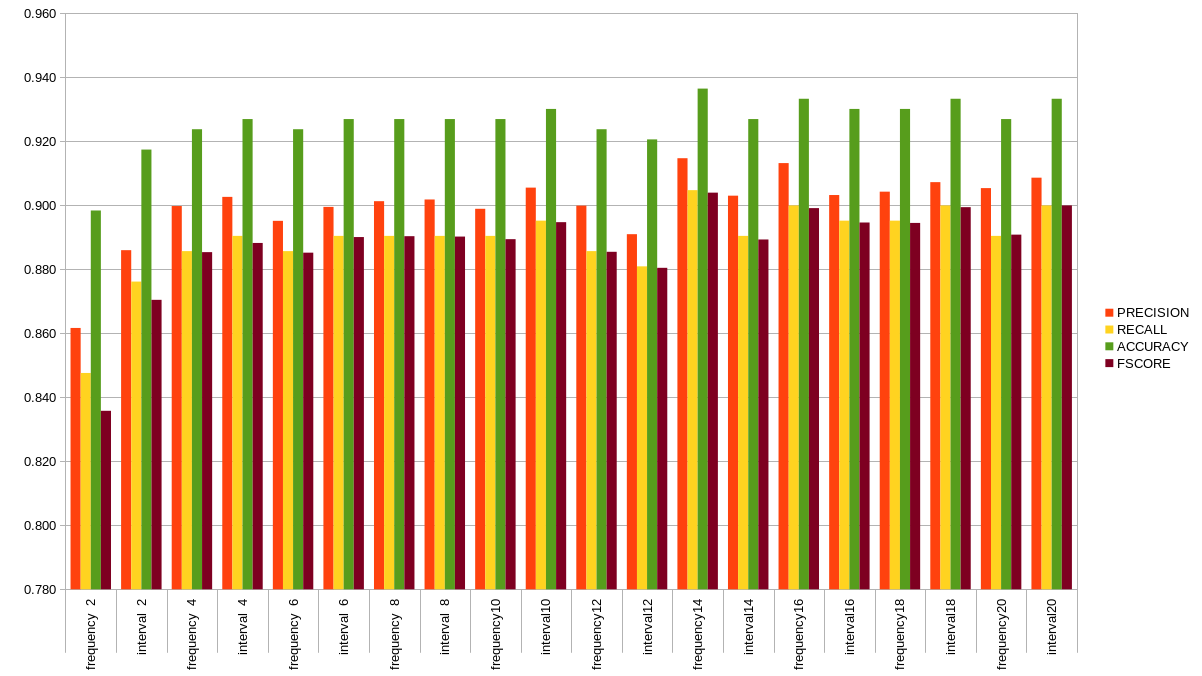
\includegraphics[width=1.0\linewidth]{disc_seeds.png}
	\caption[Wyniki klasyfikatora dla różnych metod dyskretyzacji. Zbiór seeds.]{Wyniki klasyfikatora dla różnych metod dyskretyzacji. Zbiór seeds.}
	\label{fig:disc_seeds}
\end{figure}

\subsection{Zbiór ecoli}
Poniżej przedstawiono porównanie metod dyskretyzacji w wynikach poszczególnych klasyfikatorów. Wyniki przedstawiają dane obliczone przy użyciu kroswalidacji stratyfikowanej oraz uśredniania ważonego.

\begin{table}[H]
\centering
\caption{Tabela zbiór ecoli.}
\label{table-ecoli}
\begin{tabular}{llrrrr}
METHOD    & SIZE & PREC & RECALL & ACCURACY & FSCORE \\
frequency & 2    & nan  & 0.721  & 0.913    & nan    \\
interval  & 2    & nan  & 0.712  & 0.911    & nan    \\
frequency & 4    & nan  & 0.768  & 0.927    & nan    \\
interval  & 4    & nan  & 0.803  & 0.941    & nan    \\
frequency & 6    & nan  & 0.809  & 0.945    & nan    \\
interval  & 6    & nan  & 0.815  & 0.945    & nan    \\
frequency & 8    & nan  & 0.794  & 0.942    & nan    \\
interval  & 8    & nan  & 0.782  & 0.940    & nan    \\
frequency & 10   & nan  & 0.774  & 0.934    & nan    \\
interval  & 10   & nan  & 0.765  & 0.934    & nan    \\
frequency & 12   & nan  & 0.771  & 0.935    & nan    \\
interval  & 12   & nan  & 0.779  & 0.938    & nan    \\
frequency & 14   & nan  & 0.762  & 0.933    & nan    \\
interval  & 14   & nan  & 0.756  & 0.932    & nan    \\
frequency & 16   & nan  & 0.744  & 0.926    & nan    \\
interval  & 16   & nan  & 0.756  & 0.931    & nan    \\
frequency & 18   & nan  & 0.753  & 0.926    & nan    \\
interval  & 18   & nan  & 0.744  & 0.924    & nan    \\
frequency & 20   & nan  & 0.732  & 0.919    & nan    \\
interval  & 20   & nan  & 0.756  & 0.926    & nan   
\end{tabular}
\end{table}
\begin{figure}[H]
	\centering
		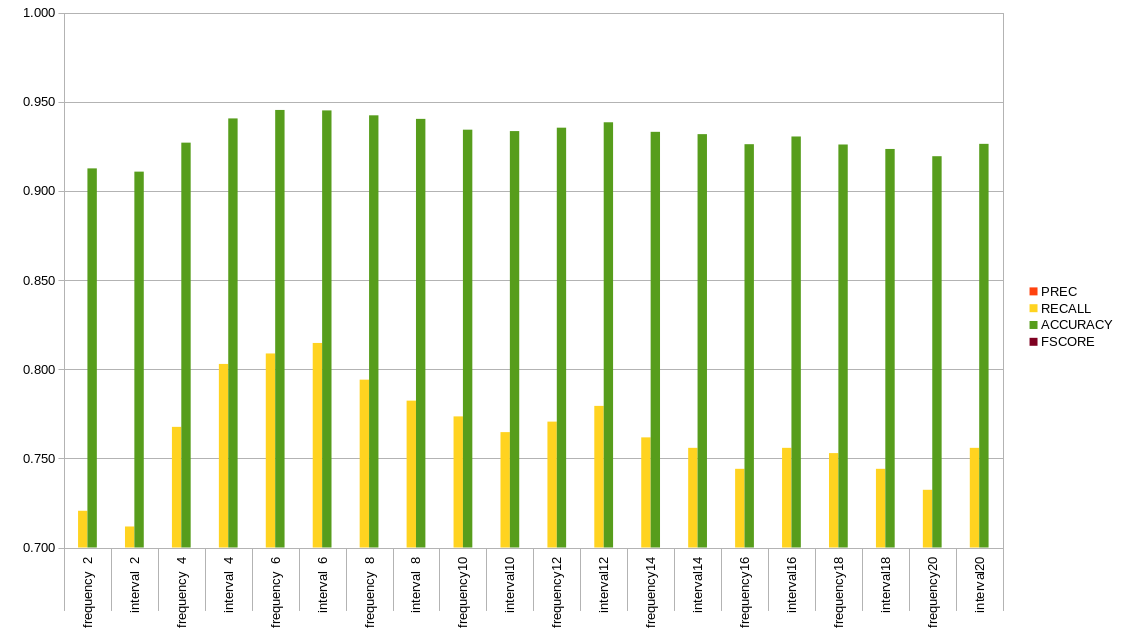
\includegraphics[width=1.0\linewidth]{disc_ecoli.png}
	\caption[Wyniki klasyfikatora dla różnych metod dyskretyzacji. Zbiór ecoli.]{Wyniki klasyfikatora dla różnych metod dyskretyzacji. Zbiór ecoli.}
	\label{fig:disc_ecoli}
\end{figure}

\subsection{Zbiór ukm}
Poniżej przedstawiono porównanie metod dyskretyzacji w wynikach poszczególnych klasyfikatorów. Wyniki przedstawiają dane obliczone przy użyciu kroswalidacji stratyfikowanej oraz uśredniania ważonego.

\begin{table}[H]
\centering
\caption{Tabela zbiór ukm.}
\label{table-ukm}
\begin{tabular}{llrrrr}
METHOD    & SIZE & PREC  & RECALL & ACCURACY & FSCORE \\
frequency & 2    & nan   & 0.574  & 0.773    & nan    \\
interval  & 2    & nan   & 0.623  & 0.800    & nan    \\
frequency & 4    & 0.788 & 0.746  & 0.857    & 0.744  \\
interval  & 4    & 0.845 & 0.826  & 0.905    & 0.824  \\
frequency & 6    & 0.823 & 0.803  & 0.891    & 0.801  \\
interval  & 6    & 0.864 & 0.851  & 0.917    & 0.851  \\
frequency & 8    & 0.866 & 0.851  & 0.917    & 0.852  \\
interval  & 8    & 0.867 & 0.849  & 0.917    & 0.847  \\
frequency & 10   & 0.855 & 0.846  & 0.914    & 0.845  \\
interval  & 10   & 0.862 & 0.841  & 0.915    & 0.839  \\
frequency & 12   & 0.863 & 0.841  & 0.911    & 0.840  \\
interval  & 12   & 0.861 & 0.844  & 0.913    & 0.842  \\
frequency & 14   & 0.870 & 0.849  & 0.917    & 0.849  \\
interval  & 14   & nan   & 0.849  & 0.918    & nan    \\
frequency & 16   & 0.842 & 0.828  & 0.905    & 0.827  \\
interval  & 16   & 0.841 & 0.823  & 0.902    & 0.823  \\
frequency & 18   & 0.835 & 0.821  & 0.901    & 0.820  \\
interval  & 18   & 0.839 & 0.815  & 0.900    & 0.814  \\
frequency & 20   & 0.831 & 0.810  & 0.897    & 0.811  \\
interval  & 20   & 0.843 & 0.823  & 0.902    & 0.821 
\end{tabular}
\end{table}
\begin{figure}[H]
	\centering
		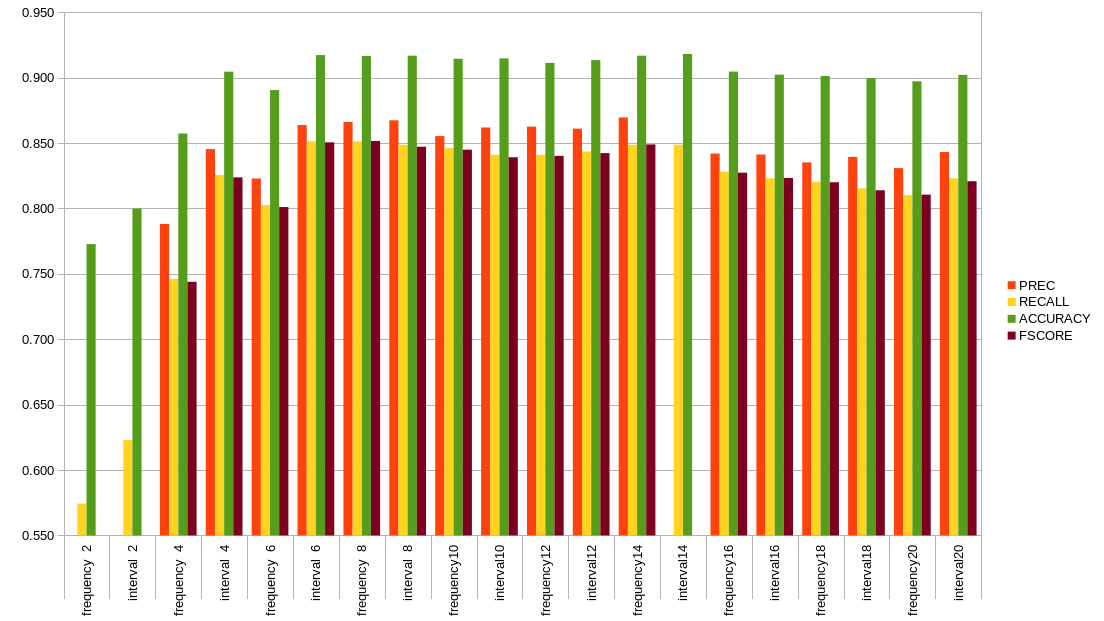
\includegraphics[width=1.0\linewidth]{disc_ukm.png}
	\caption[Wyniki klasyfikatora dla różnych metod dyskretyzacji. Zbiór ukm.]{Wyniki klasyfikatora dla różnych metod dyskretyzacji. Zbiór ukm.}
	\label{fig:disc_ukm}
\end{figure}

\section{Porównanie metod kroswalidacji}
Poniżej przedstawiono wyniki klasyfikatorów obliczone różnymi typami kroswalidacji. Dodatkowo wybrano jedynie najlepsze klasyfikatory spośród wszystkich, które wykorzystywały częstotliwością metodę dyskretyzacji. Wyniki klasyfikatorów uśredniono za pomocą średniej ważonej.

\begin{table}[H]
\centering
\caption{Tabela kroswalidacja.}
\label{table-cross}
\begin{tabular}{lllllrrrr}
NAME  & DATASET   & CROSS      & AVG & SIZE & PREC  & RECALL & ACCURACY & FSCORE \\
ukm   & frequency & stratified & w   & 8    & 0.866 & 0.851  & 0.917    & 0.852  \\
ukm   & frequency & cross      & w   & 8    & 0.865 & 0.850  & 0.914    & 0.850  \\
ecoli & frequency & stratified & w   & 6    & nan   & 0.809  & 0.945    & nan    \\
ecoli & frequency & cross      & w   & 6    & nan   & 0.852  & 0.945    & nan    \\
seeds & frequency & stratified & w   & 14   & 0.915 & 0.905  & 0.937    & 0.904  \\
seeds & frequency & cross      & w   & 14   & 0.900 & 0.890  & 0.925    & 0.890 
\end{tabular}
\end{table}
\begin{figure}[H]
	\centering
		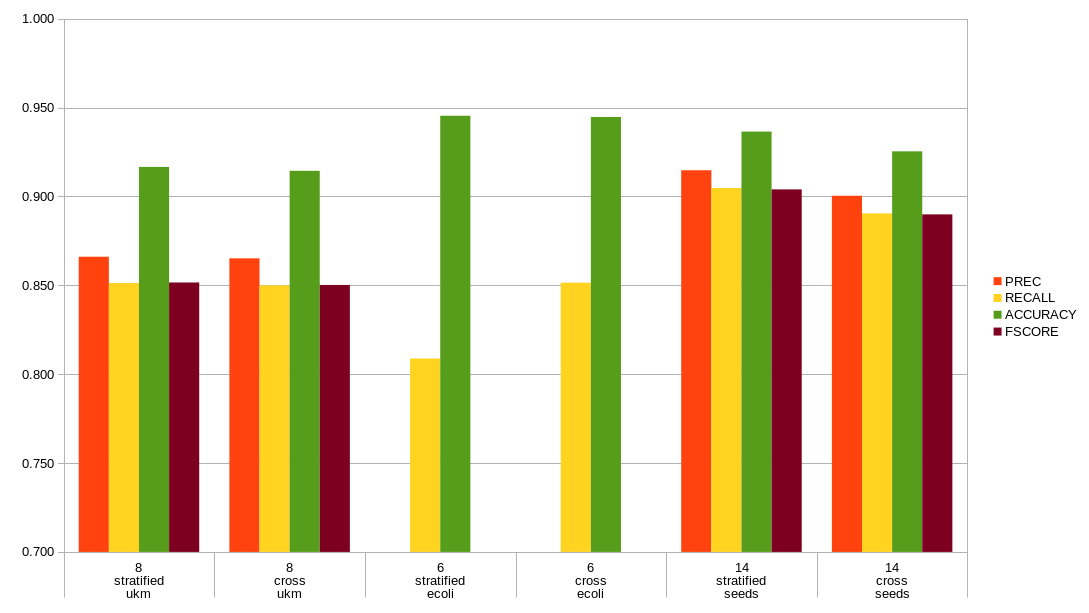
\includegraphics[width=1.0\linewidth]{cross.png}
	\caption[Wyniki klasyfikatora dla różnych metod kroswalidacji.]{Wyniki klasyfikatora dla różnych metod kroswalidacji.}
	\label{fig:cross}
\end{figure}

\section{Porównanie metod uśredniania statystyk}

Poniżej przedstawiono wyniki klasyfikatorów obliczone różnymi metodami uśredniania statystyk. Dodatkowo wybrano jedynie najlepsze klasyfikatory spośród wszystkich, które wykorzystywały częstotliwością metodę dyskretyzacji oraz kroswalidację stratyfikowaną.

\begin{table}[H]
\centering
\caption{Tabela statystyki.}
\label{table-stats}
\begin{tabular}{lllllrrrr}
NAME  & DATASET   & CROSS      & AVG & SIZE & PREC  & RECALL & ACCURACY & FSCORE \\
seeds & frequency & stratified & w   & 14   & 0.915 & 0.905  & 0.937    & 0.904  \\
seeds & frequency & stratified & u   & 14   & 0.915 & 0.905  & 0.937    & 0.904  \\
seeds & frequency & stratified & g   & 14   & 0.936 & 0.965  & 0.905    & 0.950  \\
ecoli & frequency & stratified & u   & 6    & nan   & 0.524  & 0.952    & nan    \\
ecoli & frequency & stratified & w   & 6    & nan   & 0.809  & 0.945    & nan    \\
ecoli & frequency & stratified & g   & 6    & 0.848 & 0.944  & 0.809    & 0.893  \\
ukm   & frequency & stratified & u   & 8    & 0.878 & 0.846  & 0.926    & 0.855  \\
ukm   & frequency & stratified & w   & 8    & 0.866 & 0.851  & 0.917    & 0.852  \\
ukm   & frequency & stratified & g   & 8    & 0.920 & 0.920  & 0.851    & 0.919 
\end{tabular}
\end{table}
\begin{figure}[H]
	\centering
		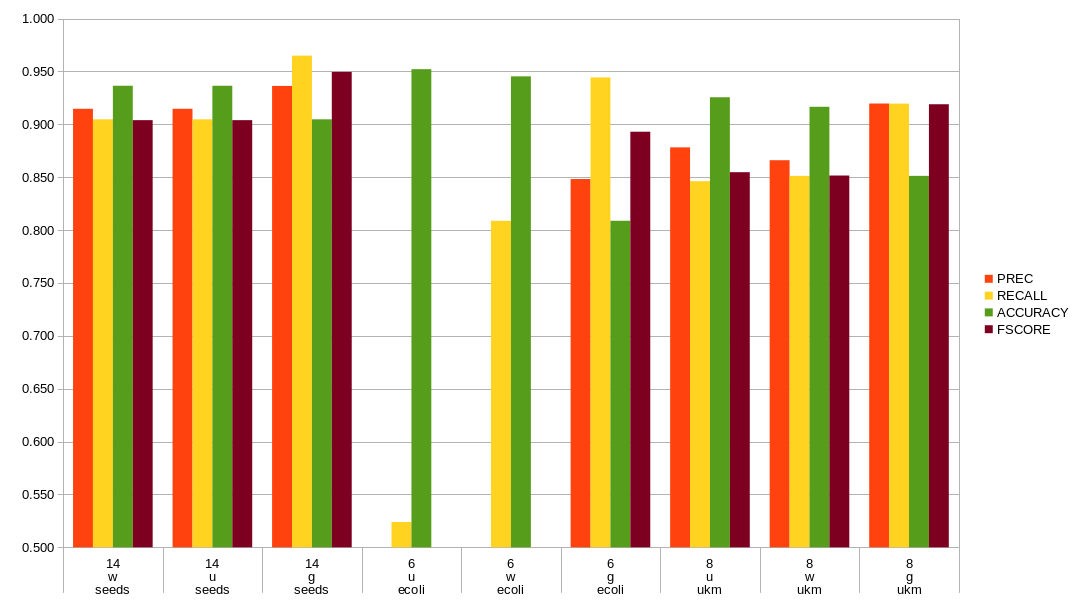
\includegraphics[width=1.0\linewidth]{stats.png}
	\caption[Wyniki klasyfikatora dla różnych metod obliczania statystyki.]{Wyniki klasyfikatora dla różnych metod obliczania statystyki.}
	\label{fig:stats}
\end{figure}

\section{Rozkład normlany}

Poniżej przedstawiono wyniki klasyfikatorów z zastosowaną dyskretyzacją w porównaniu do tych które używały prawdopodobieństwa z rozkładu Gaussa. Dodatkowo wybrano jedynie najlepsze klasyfikatory spośród wszystkich, które wykorzystywały częstotliwością metodę dyskretyzacji oraz kroswalidację stratyfikowaną. Wyniki klasyfikatorów uśredniono za pomocą średniej ważonej.

\begin{table}[H]
\centering
\caption{Tabela dane ciągłe.}
\label{table-norm}
\begin{tabular}{lllllrrrr}
NAME  & DATASET   & CROSS      & AVG & SIZE & PREC  & RECALL & ACCURACY & FSCORE \\
seeds & frequency & stratified & w   & 14   & 0.915 & 0.905  & 0.937    & 0.904  \\
seeds & norm      & stratified & w   & -    & 0.902 & 0.876  & 0.917    & 0.877  \\
ecoli & frequency & stratified & w   & 6    & nan   & 0.809  & 0.945    & nan    \\
ecoli & norm      & stratified & w   & -    & nan   & 0.412  & 0.680    & nan    \\
ukm   & frequency & stratified & w   & 8    & 0.866 & 0.851  & 0.917    & 0.852  \\
ukm   & norm      & stratified & w   & -    & 0.880 & 0.864  & 0.924    & 0.864 
\end{tabular}
\end{table}
\begin{figure}[H]
	\centering
		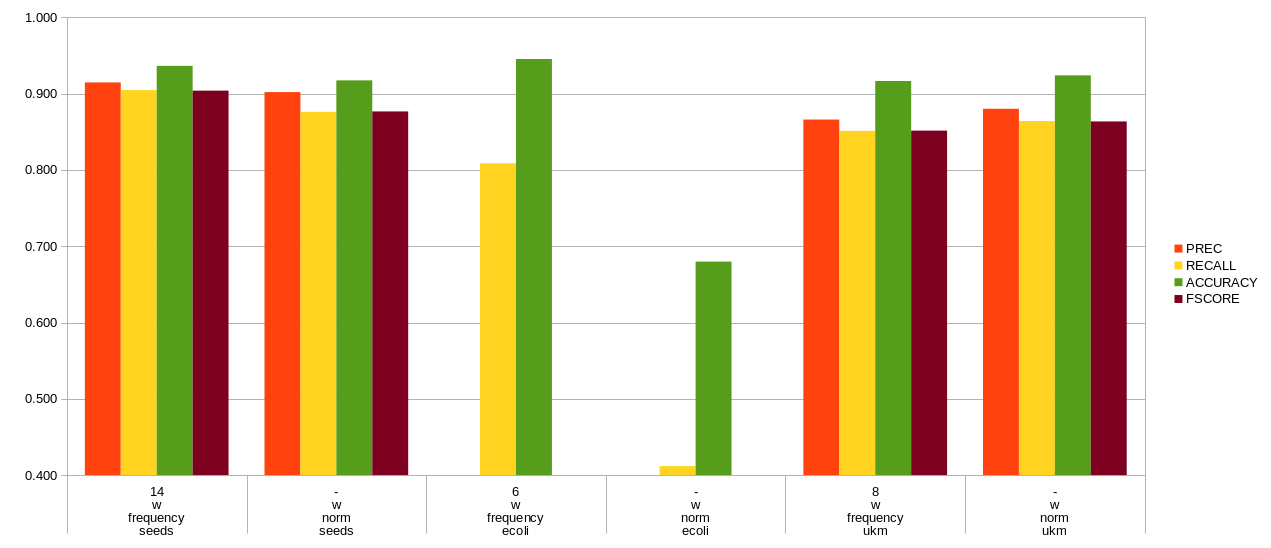
\includegraphics[width=1.0\linewidth]{norm.png}
	\caption[Porównanie wyników dyskretnych z wartościami ciągłymi.]{Porównanie wyników dyskretnych z wartościami ciągłymi.}
	\label{fig:norm}
\end{figure}
